\chapter{Evolution of Massive Stars in Isolation}\label{chap:single_star_evolution}

Stars with $M \leq 2$ M$_{\odot}$, $2 < M \leq 8$ M$_{\odot}$ and $M > 8$ M$_{\odot}$ are classified as low-, intermediate-, and high-mass, respectively. Despite the inherent rarity predicted by the initial mass function (IMF, see e.g. \cite{chabrier2005initial, dib2018emergence}), massive stars play a key role in the evolution of the Universe. They are the main source of UV radiation and heavy elements. They serve as a significant source of mixing and turbulence in the interstellar medium (ISM) of galaxies through a combination of winds, outflows, expanding HII regions, and supernova explosions. Galactic dynamos are powered by turbulence in conjunction with differential rotation. Cosmic rays are accelerated by the interaction of galactic magnetic fields and supernova shock fronts. The ISM is primarily heated by cosmic rays, UV radiation, and the dissipation of turbulence, whereas it is finally cooled by heavy metals present in dust, molecules, and in atomic/ionic form. Therefore, massive stars have a significant impact on galaxies' physical, chemical, and morphological structure \citep{kennicutt2005role}. However, the physical mechanisms behind the birth, development, and demise of massive stars remain elusive in comparison with low-mass stars \citep{zinnecker2007toward}. 


\section{Timescales of Stellar Evolution}

The fundamental timescales of stellar evolution are the dynamical ($t_{dyn}$), thermal ($t_{th}$), and nuclear timescales ($t_{nucl}$). The dynamical timescale is the characteristic time required for a star to collapse under its own gravitational force in the absence of internal pressure:

\begin{equation}
    t_{dyn} = \sqrt{\frac{R^3}{GM}} \sim 0.02 \left( \frac{R}{R_{\odot}} \right)^{3/2} \left( \frac{M}{M_{\odot}}\right)^{1/2} \; \text{days},
\end{equation}\label{eq:dynamical_timsecale}

where $R$ and $M$ are the star's radius and mass. It is a period on which a star might expand or contract if its hydrostatic equilibrium were disrupted, e.g. in case of sudden mass loss.

Thermal (or Kelvin-Helmholtz) timescale indicates how quickly changes in a star's thermal structure may occur. It is therefore also the period on which a star responds when a its thermal equilibrium is disturbed:

\begin{equation}
    t_{th} = \frac{G M^2}{2RL} \sim 1.5 \times 10^7 \left( \frac{M}{M_{\odot}} \right)^{2} \frac{R_{\odot}}{R} \frac{L_{\odot}}{L} \; \text{yr},
\end{equation}\label{eq:thermal_timsecale}

where L is the star's luminosity.

Finally, the nuclear timescale corresponds to the time required for the star to exhaust its nuclear fuel supply at its current luminosity: 

\begin{equation}
    t_{nucl} = \frac{\phi M_{nucl} c^2}{L} \sim 10^{10} \frac{M}{M_{\odot}} \frac{L_{\odot}}{L} \; \text{yr},,
\end{equation}\label{eq:nuclear_timsecale}

where $\phi$ is the efficiency of nuclear energy production, $M_{nuc}$ is the amount of mass available as fuel, and $c$ is the light speed. For core hydrogen burning, $\phi = 0.007$ and $M_{nucl} \sim 0.1 M$.

Typically $t_{nucl} >> t_{th} >> t_{dyn}$, while assuming a mass-luminosity relation of $L \propto M^{\alpha}$, with empirically $\alpha \sim 3-4$ \citep{eker2015main}, it follows that massive stars live shorter and evolve faster than low-mass stars.

\section{Hertzsprung-Russell diagram}

The evolution of a star in isolation, namely single star evolution, is predominantly determined by the stellar mass. In their attempt to achieve hydrostatic and thermal equilibrium, stars generate temperatures and pressures that allow for nuclear burning. The cycles of nuclear burning and fuel exhaustion regulate the evolution of a star and set the various phases during the stellar lifetime. These burning cycles can be viewed as long-lived but transient disruptions to a star's (or at least its core's) inexorable shrinkage under the effect of gravity. The virial theorem dictates this contraction is caused by the fact that stars are hot and lose energy through radiation. 

The Hertzsprung-Russell (HR) diagram in \cref{fig:HR_massive_stars} shows three evolutionary tracks for massive stars. The black circles correspond to the Zero Age Main Sequence (ZAMS) and the Terminal Age Main Sequence (TAMS). At ZAMS, the star having started the hydrogen burning in its core, achieves thermal equilibrium (TE), $L_{nuc}/L =1$, while TAMS is defined as the core hydrogen exhaustion point. Additionally, the black squares represent the start and end of helium burning in the core, respectively. In both cases the end of nuclear burning in the core has defined as the point when hydrogen and helium core mass fractions are $< 0.01$, respectively. Finally, between TAMS and the ignition of helium, there is a short-lived phase called Hertzsprung gap branch, where hydrogen burning occurs in a shell around the core. 

\begin{figure}[H]
    \centering
    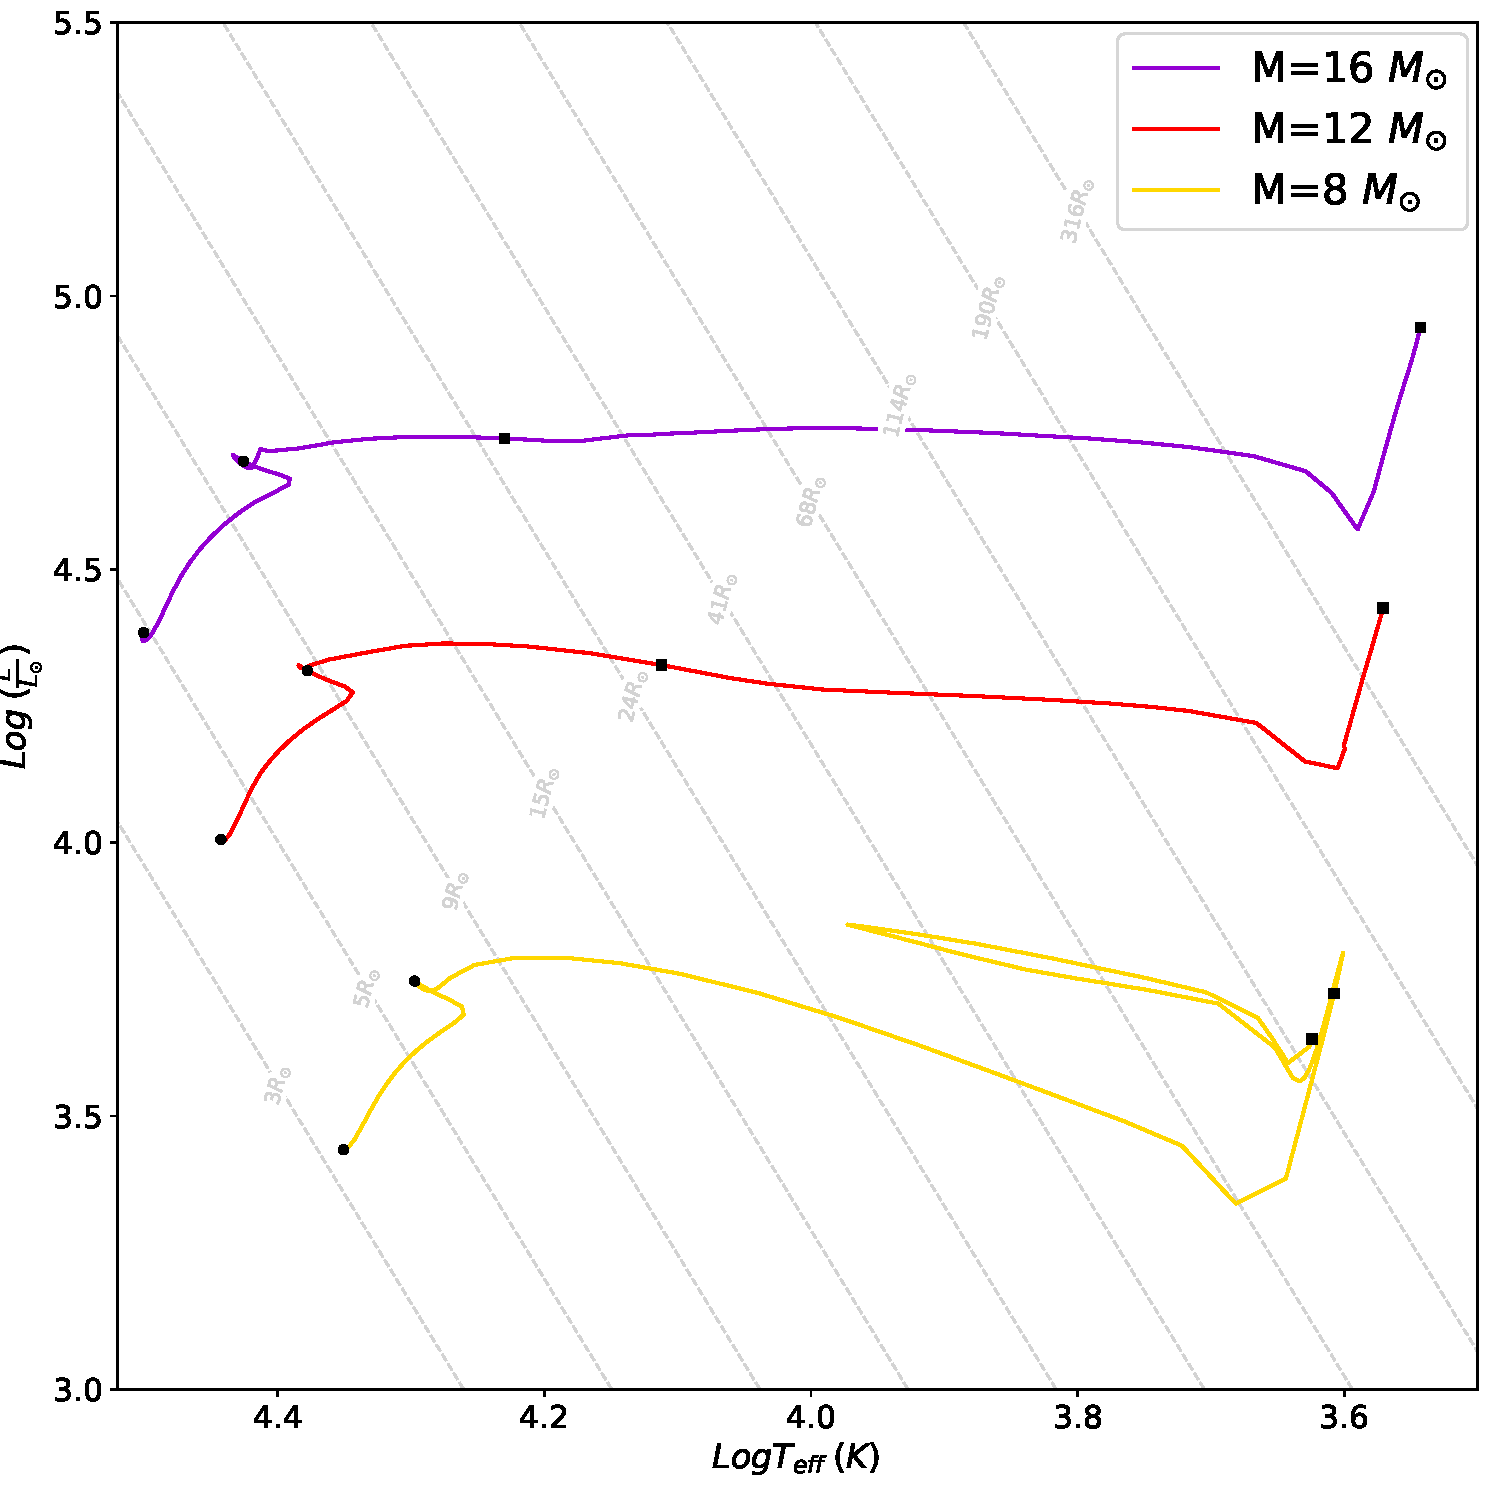
\includegraphics[width=0.9\textwidth]{Thesis/graphs/HR_massive_stars.pdf}
    \caption{Hertzsprung-Russell diagram. Evolutionary tracks for three stars in the HR-diagram with masses 9, 12 and 15 M$_{\odot}$ at solar metallicity until the end of Hellium burning. Specific moments in the evolution of the stars are noted by black circles and squares as explained in the text. The tracks are calculated with MESA (cite to be). The dashed lines show lines of constant radii by means of the Stefan–Boltzmann law.}
    \label{fig:HR_massive_stars}
\end{figure}

During the MS, hydrogen is fused into $^4$He. Independently on the ongoing reaction channel (pp or CNO), the luminosity of the star increases during this phase, (L$\,\propto\,\mu^{4}\,M^3$), due to the change in the core's composition ($\mu$ increases). Nevertheless, the way in which the star evolves through the MS-phase depends on its mass. Stars with masses M\,$\geq$\,1.3\,M$_\odot$, consequently massive stars too, are driven by the CNO-cycle ($\epsilon_{CNO}\,\propto\,\rho_{c}T^{18}_{c}$). As the luminosity increases over time, the energy produced in the core needs to increase too, in order to maintain TE. However, due to the high dependence on the central temperature of the CNO-cycle, a small change of T$_c$ will have a tremendous effect on the energy production rate $\epsilon_{CNO}$, which would take out the star from HE and TE. Thus, T$_c$ needs to remain almost constant in time. The ideal gas law implies that $\frac{P_c}{\rho_c} \propto \frac{T_c}{\mu}$, hence while $\mu$ increases, in order to decrease the pressure inside the core, the envelope expands on nuclear time-scale. Stars driven by the CNO-cycle evolve through larger radii and lower T$_{eff}$ than stars driven by the pp-cycle. 

Furthermore, stars driven by the CNO-cycle have convective cores, since the energy produced is too large to be transported by radiation ($\nabla_{rad} > \nabla_{ad}$). One effect of the convection on the evolution is that the MS-lifetime is extended (H is brought from the envelope inside the core, more detailed discussion in \cref{sub:mixing}). Another effect is that as the core approaches the end of H-burning, the reactions suddenly cease in the whole core. Consequently, the energy generation rate would normally decrease due to the sudden depletion of hydrogen in the core, which also diminishes the thermostatic action of the CNO reactions, threatening the thermal equilibrium of the star. In response the temperature of the core needs to increase in order to keep the same energy generation rate, $\epsilon_{CNO}$. As a result, the pressure exerted on the core by the envelope must increase, $\frac{P_c}{\rho_c} \propto \frac{T_c}{\mu}$, leading to the contraction of the star which also leads to higher effective temperature. This is evident in the second part of the MS (see \cref{fig:HR_massive_stars}), where we observe the ``hook'' feature. 

At TAMS, where the hydrogen in the core has been depleted, hydrogen burning occurs in a shell around the core, while the central temperature is insufficient to initiate burning in the helium core. From that point on, the star enters the Hertzsprung gap branch. The core contracts in $t_{th}$ in an attempt to reach thermal equilibrium. The virial theorem indicates that half of the gravitational energy ($E_{grav}$) is converted to internal energy ($E_{int}$) raising the central temperature, while the other half is escaping as luminosity ($L_c$) from the core. Furthermore, the hydrogen burning shell around the core also produces energy via the CNO-cycle. The thermostatic behavior of the CNO-cycle indicates that the burning shell must maintain thermal equilibrium by remaining at a relatively constant temperature. Because contraction of the burning shell would result in heating, the radius of the burning shell must also stay fairly constant. As the core contracts, sp does the shell and so the pressure in the burning shell increases. As a result, the overlaying envelope's pressure must drop, causing the layers above the shell to expand, $\frac{P_{sh}}{\rho_{sh}} \propto \frac{T_{sh}}{\mu_{sh}}$. This called the mirror principle. The aforementioned behavior is evident in Fig. \ref{fig:HR_massive_stars}, as the stars move towards bigger radius and lower effective temperature. An important thing to mention is that during this phase the temperature in the core is raising up and should not be confused with the effective temperature. As the star moves towards lower effective temperatures, the opacity ($\kappa$) in the envelope raises, thus the energy transport through radiation becomes less efficient ($\nabla_{rad} \propto \kappa$), while gradually the envelope becomes convective.

\begin{comment}
A significant fraction of the energy from these two sources acts as the work applied towards the envelope leading to the expansion of the latter under hydrostatic equilibrium, while the expansion itself results to the envelope temperature being reduced. Simultaneously, the abundance of hydrogen in the shell is reducing making the shell gradually thinner, while the produced helium is adding gradually mass to the helium core speeding up its contraction.
\end{comment}

Stars of less than $12$M$_{\odot}$ reach each effective temperatures as low as ($10^{3.7}$K) 5000K before helium ignition. At this moment, they begin to ascend the red giant branch (RGB), which is accompanied by a significant rise in luminosity and radius. Due to the low effective temperature the opacity of the envelope rises and the latter becomes gradually convective. The prohibited zone of the HR-diagram is located to the right of the RGB, where hydrostatic equilibrium cannot be established. Any star in this zone will travel quickly towards the RGB. The red giant star has a compact core and an extensive envelope that extends hundreds of solar radii. When the temperature in the core exceeds $T_c \sim 10^8 K$, helium core burning begins, and the red giant phase ends. For stars with $M \geq 12$M$_{\odot}$, helium ignites before the effective temperature has dropped to a few thousand Kelvin. The stellar tracks for stars of less than $12$M$_{\odot}$ form a loop on the HR-diagram during helium burning, also known as the horizontal branch. The loop is accompanied by a drop and increase in the stellar radius. As the blazing front advances from the core to a shell enclosing the core, the star's outer layers expand again, and the evolution continues.

\begin{comment}
The important difference here is that there is a shell in which hydrogen burning takes places via the CNO-cycle. Consequently, the expansion of the layers around the core will result to the increase of the pressure that is exerted by the latter towards that shell. The thermostatic behavior of the CNO-cycle once again tries to maintain the thermal equilibrium, $T_{sh} \sim const.$ in the shell, and because $\frac{P_{sh}}{\rho_{sh}} \propto \frac{T_{sh}}{\mu_{sh}}$ the pressure by the envelope towards the hydrogen burning shell must increase. This leads to the envelope's contraction and consequently to the reduction of the luminosity $L$ as can be seen in Fig. \ref{fig:HR2}, which is still determined by the conditions in the photosphere because of the convective envelope. The contraction takes place until point {\it F}, but it is evident that the rate of the contraction becomes lower as the star moves towards {\it F}. In reality the temperature in the envelope slowly rises as the star reaches the end of the red-giant branch (transition from the red line to the blue line), thus the opacity also rises and the envelope becomes gradually less convective and more radiative. This is happening because not all the layers from the hydrogen burning shell and above are convective, but there is a small part at the bottom of the envelope that is still radiative. Hence, the helium burning acts now as a second source of energy inside the star. As the latter moves towards the transition point is already in thermal equilibrium and the virial theorem indicates that as the envelope contracts must rise its internal energy, thus rise its temperature. Consequently, the radiative layers above the core (not the hydrogen burning shell) are gradually heated erasing the convection from inside towards the surface of the star. From the transition point on the star enters the blue loop with a radiative envelope, which keeps contracting but the contraction is slowly decelerating, and a gradually increasing effective temperature. Hence, the luminosity starts to rise, because has a stronger dependence on the effective temperature than on the radius ($L \propto R^2 T_{eff}^4$). This is evident in Fig. \ref{fig:HR2}.

As a result, stars go through expansion and contraction phases during their lives. The change in the star's physical radius occurs at different timescales depending on the physical mechanism buried beneath these processes. For example, in nuclear timescale ($t_{nuc}$, see \eqref{eq:nuclear_timsecale}), stars expand throughout the main sequence (MS), but in thermal timescale ($t_{th}$, see \eqref{eq:thermal_timsecale}), stars expand during the H-shell burning phase.
\end{comment}



\section{Stellar Winds}



\section{Internal Mixing}\label{sub:mixing}

Even though the overall stellar evolution is only slightly affected by the initial chemical composition, a variety of internal mixing process can impact the life cycle, particularly of massive ($M>8$ M$_{\odot}$), stars \citep{langer2012presupernova}. Apart from convection, convective overshooting, semiconvection, and rotationally induced mixing are the most important internal mixing process \citep{schootemeijer2019constraining} and are still poorly understood. 

\subsection{Convective Overshooting}

Convective overshooting refers to the process of mixing beyond the boundaries of convective regions, which can occur when convective cells penetrate into radiative regions due to their non-zero velocity \citep{alongi1993evolutionary,brott2011rotating,schootemeijer2019constraining}. In stars with convective cores, e/g/ intermediate and massive stars, the size of the core is effectively enlarged through mechanisms such as convective core overshooting. This overshooting brings additional hydrogen into the core of the star and therefore directly impacts the final He core mass and main-sequence (MS) lifetime as well as the evolution of the stars after the MS.


